
\textbf{\textit{Detector Response and Statistical Treatment}}---While neutrinos produced by SNe do not have sufficient energy to be individually resolved by neutrino telescopes, the large number arriving together generates a temporally localized increase in the detector's noise rate.
In order to simulate the light yield from signal the previously described models would produce, we use the \texttt{ASTERIA}~\cite{spencer_griswold_2020_3926835} software.
This program uses parameteriations of \texttt{GEANT4} photon yields from neutrino interactions and photon propagation to estimate the light observed for different neutrino 
In order to interface with \texttt{ASTERIA}, we use the \texttt{SNEWPY} packages, which allows us to define custom supernova fluxes.

\begin{figure*}
    \centering
    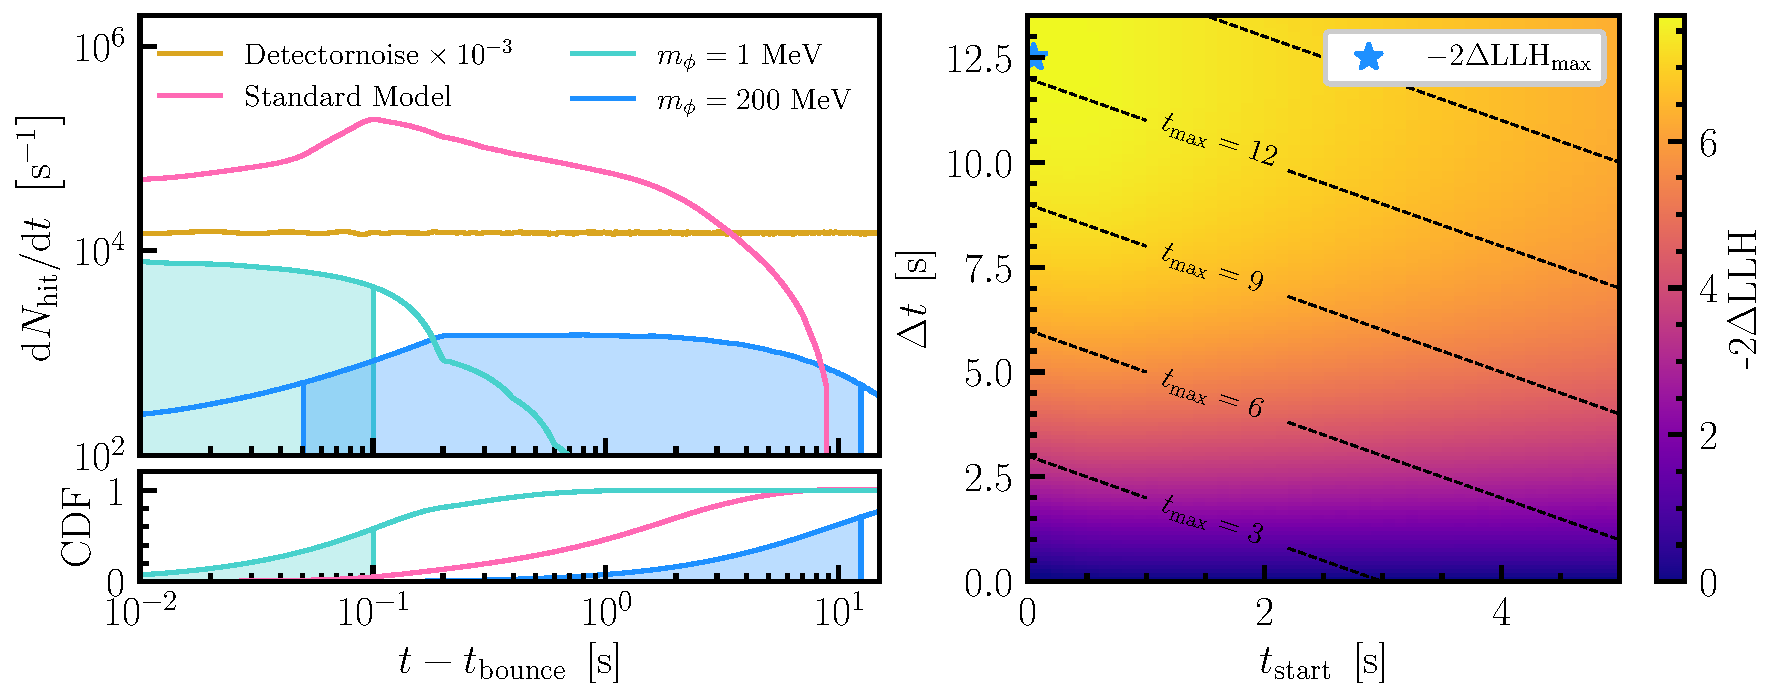
\includegraphics[width=0.95\textwidth]{figures/hits_and_likelihood.pdf}
    \caption{\textbf{\textit{Test statistic as a function of $t_{\mathrm{start}}$ and $\Delta$t.}
    }}
    \label{fig:hits_and_likelihood}
\end{figure*}